\title{Scalars Lattice Graphical Interface}
\center{author: Jérôme Rousselot}


\section{Overview}

The Scalars Lattice tool (scalati) is a cross-platform graphical interface to analyze the results of Omnet++ simulation runs. It loads all scalar files generated by a configuration, and helps the user to plot this data using the R lattice framework. Figures can be plotted on screen in a separate window, in bitmap PNG files and in vector EPS files for high resolution output. This is a tool in development and contributions are welcome.

Figure \ref{fig:scalati-complex} illustrates the current capabilities of scalati.

%
\begin{figure}[tbh]
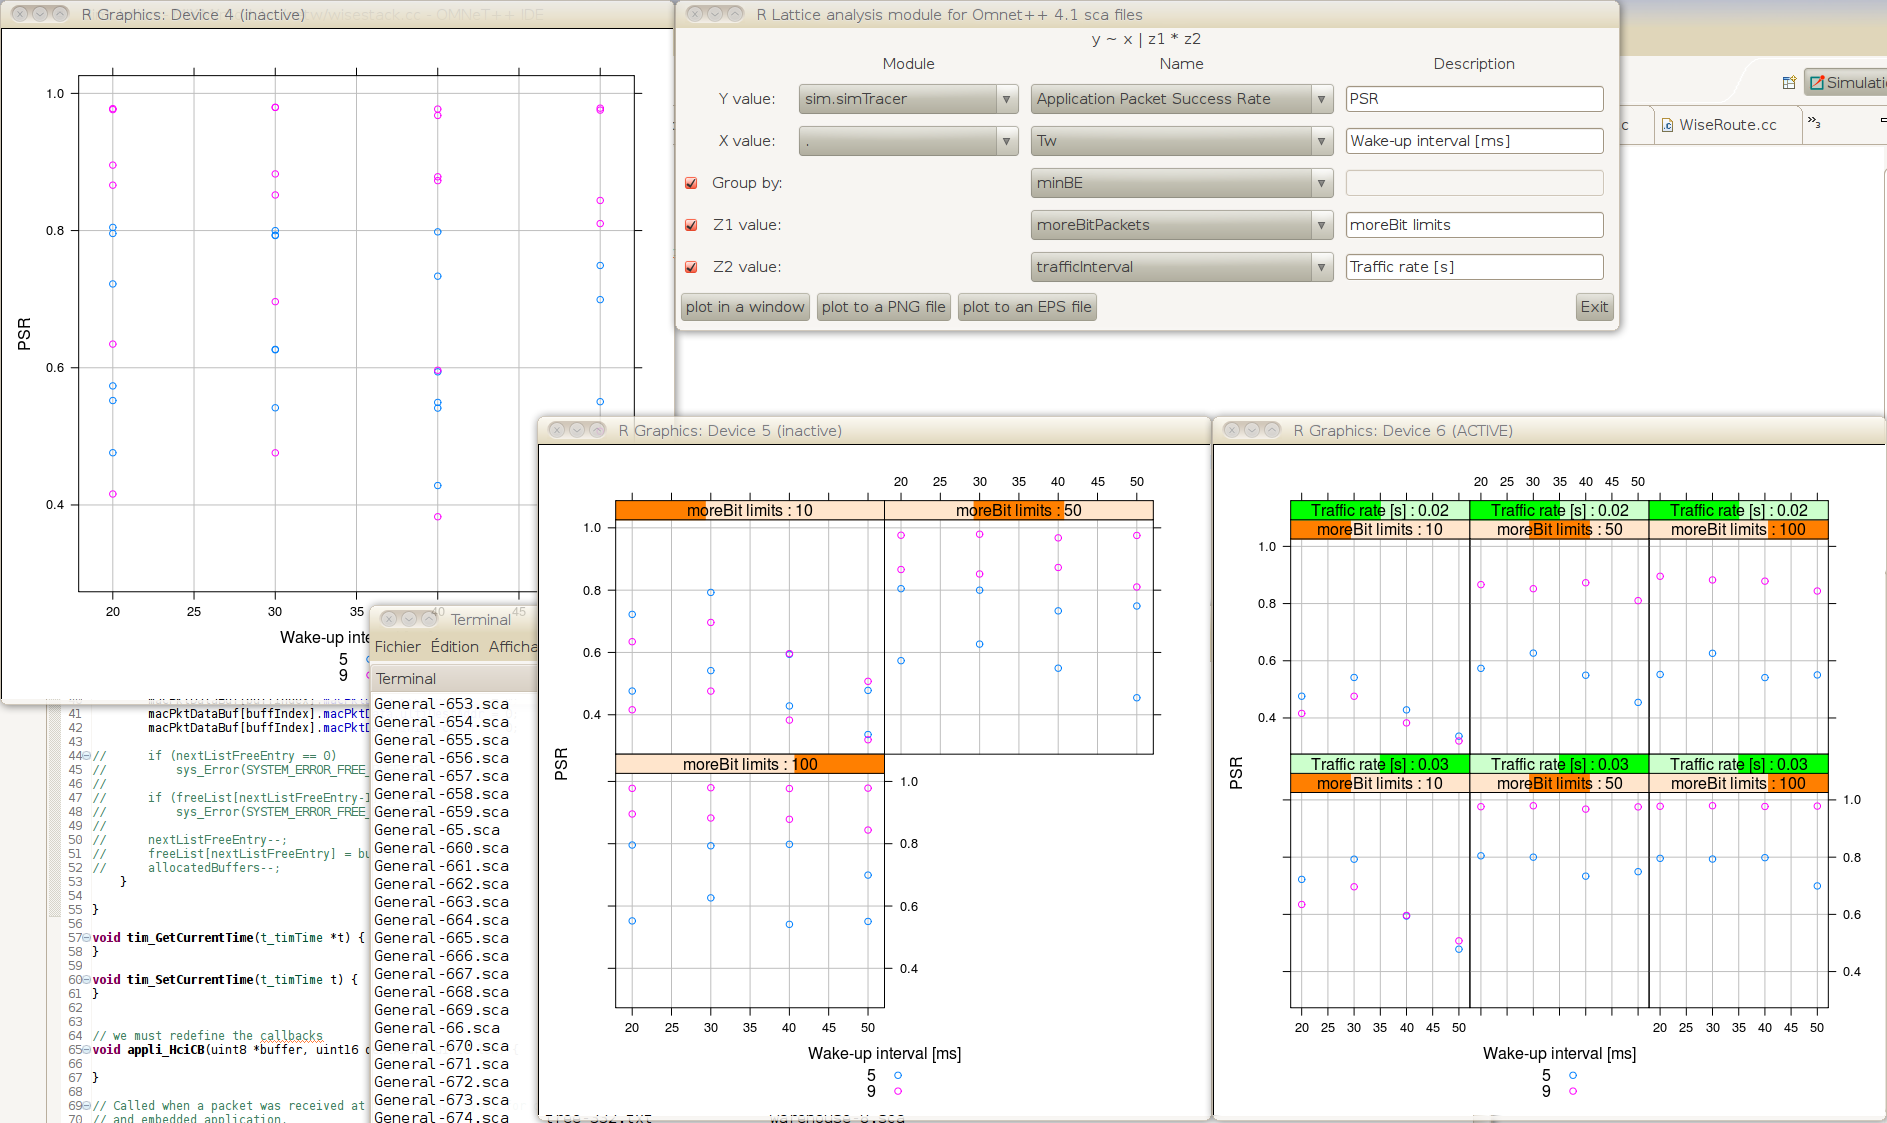
\includegraphics[width=1\columnwidth]{figures/scalati/scalati-complex_scenario.png}

\caption{\label{fig:scalati-complex}A real-life usage of scalati to identify the impact of various parameters on a metric.}

\end{figure}


\section{Installation}

scalati depends on a few R packages, which you will need to install:

\begin{itemize}
\item omnetpp
\item lattice
\item gdata
\item gWidgets
\end{itemize}

Type the following command in the R interpreter:

\begin{verbatim}
$packages.install(c("lattice", "gdata", "gWidgets"))
\end{verbatim}

Additionally, you will need at least one of: gWidgetsRGtk2 gWidgetstcltk
Use the first one under Linux, and the other under Windows and MacOS. Install with:

\begin{verbatim}
$packages.install("gWidgetsRGtk2")
\end{verbatim}

or (Windows and MacOS):

\begin{verbatim}
$packages.install("gWidgetstcltk")
\end{verbatim}

See http://wiener.math.csi.cuny.edu/pmg/gWidgets/ for more information on gWidgets, a cross-platform GUI API for R.

See http://wiki.github.com/omnetpp/omnetpp-resultfiles/omnetpp-r-package-tutorial to download and install the omnetpp package.

Once this is done, download the scalati.R file and place it in the results directory that you want to study. You must still edit scalati.R to comment out the GUI toolkit reference, depending on your platform: options(“guiToolkit”=“RGtk2”) on linux, options(“guiToolkit”=“tcltk”) on Windows and MacOS X.


\section{Step by step}

Start R in the directory where you placed “scalati.R” and type:

\begin{verbatim}
$source("scalati.R")
\end{verbatim}

Set the working directory to where the sca files to study can be found, if it is not the current directory:

\begin{verbatim}
$setwd("/home/jerome/software/omnet/omnetpp-resultfiles/R-package/inst/extdata/berdistance")
\end{verbatim}

Start the interface:

\begin{verbatim}
$scalati()
\end{verbatim}

Give the configuration name to study: type “BERDistance”

The main window appears. The first two lines let you select the fields to use as Y and X values.

Select mac as module for Y value, and its “Average BER” field. Choose special module “.” and the “berdistance” ini file iteration variable for the X value.

Generate the plot on screen:

Now, ask lattice to distinguish points depending on the channel iteration variable:

The graphic use two colors for the two channel values. We observe that the line of sight (los) channel performs much better than the non line of sight channel.

In more complex scenarios (three or four iteration variables), the Z1 and Z2 variables can be used to generate a lattice plot

\section{How to contribute}

\begin{itemize}
\item improve the wiki documentation (this page !)
\item test on other platforms: scalati is developed on linux x64. Experience, and patches/recipes to make it work with Windows XP/Vista/7 and Mac OS X are welcome.
\item add more features: options for lattice (scales parametrization, logx, logy…), multi-pages windows visualization
\item Point of contact: mailing-list / googlegroup omnetpp at http://groups.google.com/group/omnetpp/subscribe?reason=post&_done=/group/omnetpp/post?pli%3D1
\end{itemize}

\section{References}

\begin{itemize}
\item R: http://www.r-project.org
\item lattice: http://www.his.sunderland.ac.uk/~cs0her/Statistics/UsingLatticeGraphicsInR.htm
\item gWidgets: http://wiener.math.csi.cuny.edu/pmg/gWidgets/
\item traitr: http://cran.r-project.org/web/packages/traitr/index.html
\end{itemize}


